\documentclass[a4paper]{article}
\usepackage[utf8]{inputenc}
\usepackage{a4wide}
\usepackage{tikz}
\usepackage{pgffor}
\usepackage[shortlabels]{enumitem}
\usetikzlibrary{automata, positioning, arrows}
\title{An Exploration of Finite State Automata}
\author{Alan Teesdale}
\date{August 2022}
\tikzset{
	->, % makes the edges directed
	>=stealth', % makes the arrow heads bold
	node distance=3cm, % specifies the minimum distance between two nodes. Change if necessary.
	every state/.style={thick, fill=gray!10}, % sets the properties for each ’state’ node
	initial text=$ $, % sets the text that appears on the start arrow
}
\begin{document}

	\maketitle

	\section{Traffic Light}
	\begin{figure}[!h]
		\centering
		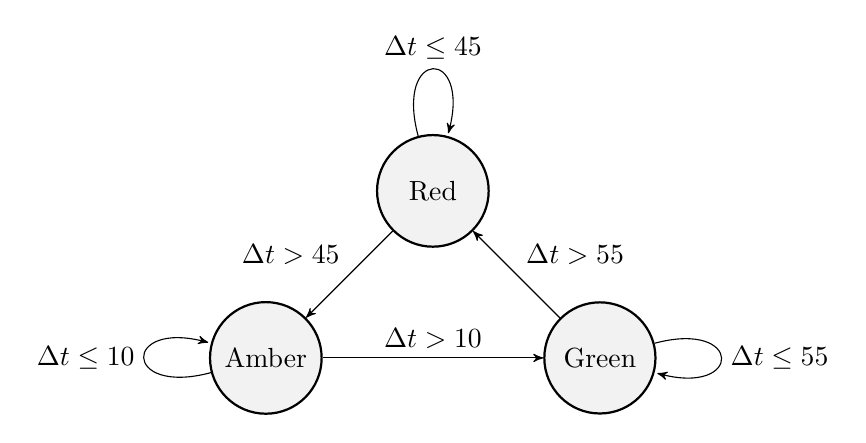
\begin{tikzpicture}
			\node[state, text width = 1.1cm, text centered] (1) {Red};
			\node[state,  text width = 1.1cm, text centered] (2) [below left of =1]{Amber};
			\node[state,  text width = 1.1cm, text centered] (3) [below right of =1]{Green};

			\draw (1) edge[above left] node{$\Delta t > 45$} (2)
				  (1) edge[loop above] node{$\Delta t \leq 45$} (1)
				  (2) edge[above] node{$\Delta t > 10$} (3)
				  (2) edge[loop left] node{$\Delta t \leq 10$} (2)
				  (3) edge[above right] node{$\Delta t > 55$} (1)
				  (3) edge[loop right] node{$\Delta t \leq 55$} (3);
		\end{tikzpicture}
		\caption{Graph showing the finite state automata where $\Delta t$ represents the number of ticks, or seconds, since the last state change.}
	\end{figure}
    \pagebreak
	\section{Decimal Parser}
	\begin{figure}[!h]
		\centering
		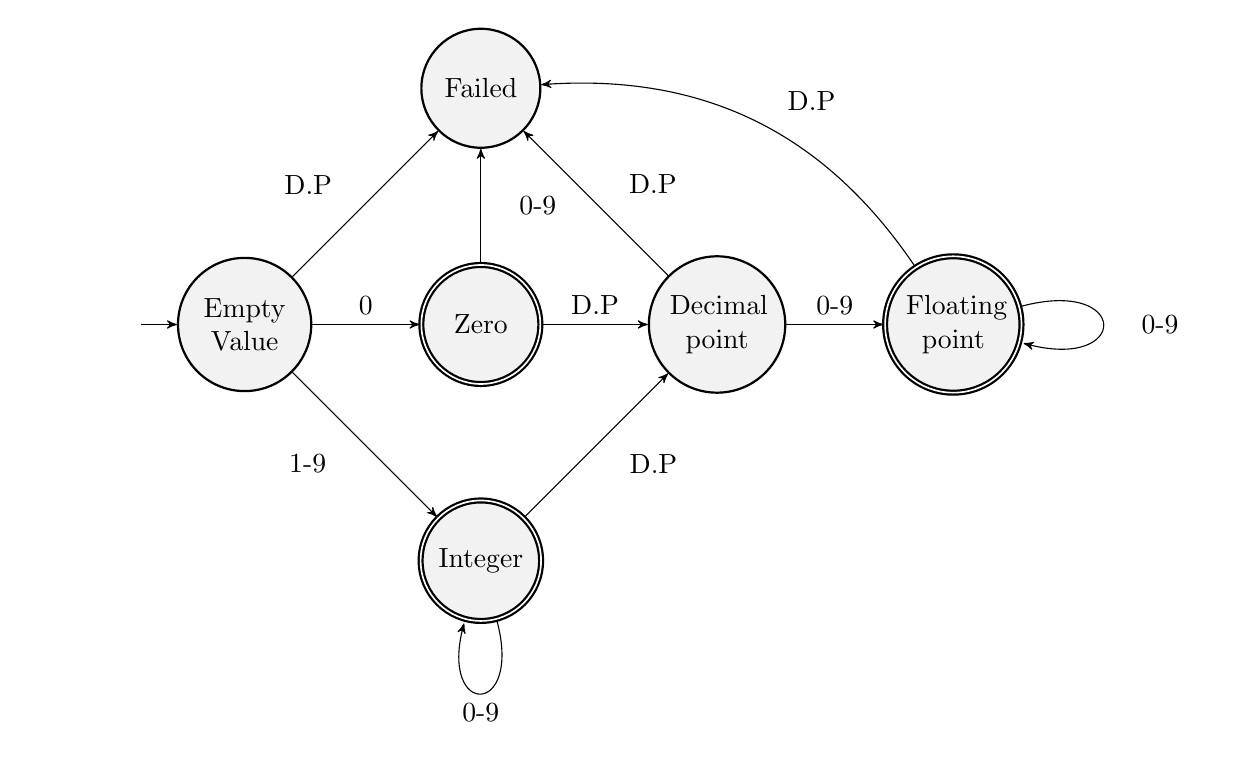
\begin{tikzpicture}[text width=1.2cm, text centered]
			\node[state, initial] (s) {Empty Value};
			\node[state, accepting] (z) [right of=s] {Zero};
			\node[state] (f) [above of=z] {Failed};
			\node[state, accepting] (di) [below of =z] {Integer};
			\node[state] (dp) [right of =z] {Decimal point};
			\node[state, accepting] (fl) [right of=dp] {Floating point};

			\draw (s) edge[above] node{0} (z)
				  (s) edge[above left] node{D.P} (f)
				  (s) edge[below left] node{1-9} (di)
				  (di) edge[loop below] node{0-9} (di)
				  (z) edge[right] node{0-9} (f)
				  (z) edge[above] node{D.P} (dp)
				  (di) edge[below right] node{D.P} (dp)
				  (dp) edge[above right] node{D.P} (f)
				  (dp) edge[above] node{0-9} (fl)
				  (fl) edge[bend right, above right] node{D.P} (f)
				  (fl) edge[loop right] node{0-9} (fl);
		\end{tikzpicture}
		\caption{A finite state machine that parses a number from a string one character at a time. The state machine ends when the final character is reached. The parse is considered a success if the ending position is on an accepting node. Any undefined behaviour, such as encountering a character not in \{`0', `1', `2', `3', `4', `5', `6', `7', `8', `9',`.'\}, is automatically assumed to be a fail.}
	\end{figure}
	\section{Letters to Digits and vice versa converter}
	\begin{tabular}{p{0.5\textwidth} | p{0.5\textwidth}}
	\subsection{Rules}
	\begin{enumerate}[start=0,label={\bfseries R$_{\arabic*}$:}]
		\item S $\rightarrow$ STRING
		\item STRING $\rightarrow$ DIGIT STRING
		\item STRING $\rightarrow$ LETTER STRING
		\item STRING $\rightarrow$ DIGIT
		\item STRING $\rightarrow$ LETTER
		\item DIGIT $\rightarrow$ LETTER
		\item LETTER $\rightarrow$ DIGIT
		\foreach \n in {0,...,9}{\item DIGIT $\rightarrow$ \n}
		\foreach \n in {A, B, C, D, E, F, G, H, I, J}{\item LETTER $\rightarrow$ \n}
	\end{enumerate} &
	\subsection{Terminal Symbols}
	$\Sigma$ = \{1, 2, 3, 4, 5, 6, 7, 8, 9, 0, A, B, C, D, E, F, G, H, I, J\}
	\subsection{Non-terminal Symbols}
	$N$ = \{STRING, DIGIT, LETTER\}
	\subsection{Finite State Machine}

		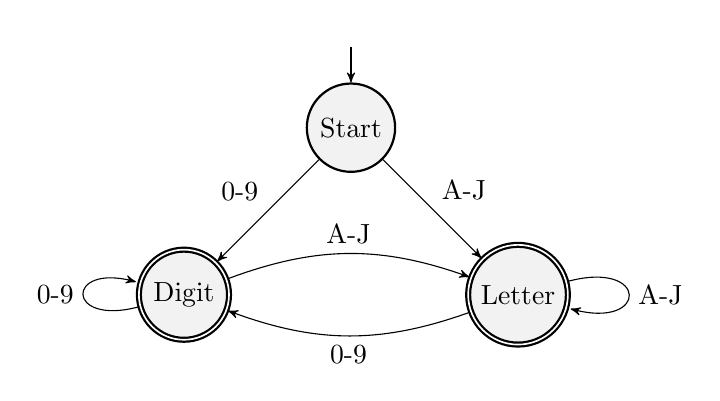
\begin{tikzpicture}
			\node[state, initial above] (s) {Start};
			\node[state, accepting] (d) [below left of=s] {Digit};
			\node[state, accepting] (l) [below right of=s] {Letter};

			\draw (s) edge[above left] node{0-9} (d)
				  (s) edge[above right] node{A-J} (l)
				  (d) edge[bend left=20, above] node{A-J} (l)
				  (l) edge[bend left=20, below] node{0-9} (d)
				  (d) edge[loop left] node{0-9} (d)
				  (l) edge[loop right] node{A-J} (l);

		\end{tikzpicture}
\end{tabular}

\end{document}

